\documentclass{article}
\usepackage[utf8]{inputenc}
\usepackage{float} % no preâmbulo
\usepackage{hyperref}
\usepackage{graphicx}
\usepackage{caption}
\usepackage{subcaption}
\usepackage{multicol}
\usepackage[margin=0.5in]{geometry}
\hypersetup{
    colorlinks=true,
    linkcolor=black,
    filecolor=black,
    urlcolor=black,
    citecolor=black,
}

\title{EA701 A - Sinais Analógicos, ADC, PWM e DAC 
}
\author{
    Raphael Salles Vitor de Souza - RA 223641 \\
    Vinicius Patriarca Miranda Miguel - RA 260731
}
\date{\today}

\begin{document}

\maketitle 

% Uncomment the following lines if you want to include a table of contents
% \renewcommand{\contentsname}{Sumário}
% \tableofcontents

\section*{Material usado}
Neste experimento, utilizamos os seguintes materiais para analisar o funcionamento do PWM e como o aumento de resistências influenciava a impedância e a forma de onda gerada pelo Raspberry Pi Pico:
\begin{multicols}{2}
\begin{itemize}
    \item BitDogLab (com Raspberry Pi Pico/Pico 2)
    \item Protoboard pequena
    \item Multímetro digital
    \item Osciloscópio digital (compartilhado, se disponível)
    \item Resistor 10~k$\Omega$ (1/4~W)
    \item Capacitor 100~nF (cerâmico)
    \item Resistor 1~k$\Omega$ (opcional, proteção)
    \item 10 jumpers macho--macho e macho--fêmea
    \item Resistores extras (1~k$\Omega$, 47~k$\Omega$) \textit{(opcional)}
    \item Capacitores extras (10~nF, 1~\textmu F) \textit{(opcional)}
\end{itemize}
\end{multicols}

\section{Leitura do Joystick}
A leitura do joystick é feita da seguinte forma, usando a função \texttt{read\_analog()}:

\begin{verbatim}
uint16_t read_analog(uint pin) {
    adc_gpio_init(pin); 
    adc_select_input(pin - 26); 
    return adc_read(); 
}
\end{verbatim}  


e usamos essa linha para imprimir os valores lidos:

\begin{verbatim}
    printf("Joystick X: %u (%.2f V) | Joystick Y: %u (%.2f V)\n", x_analog, x_volts, y_analog, y_volts);
\end{verbatim}
    

Os valores lidos estão na Figura \ref{fig:valores_joystick}:

\begin{figure}[h!]
    \centering
    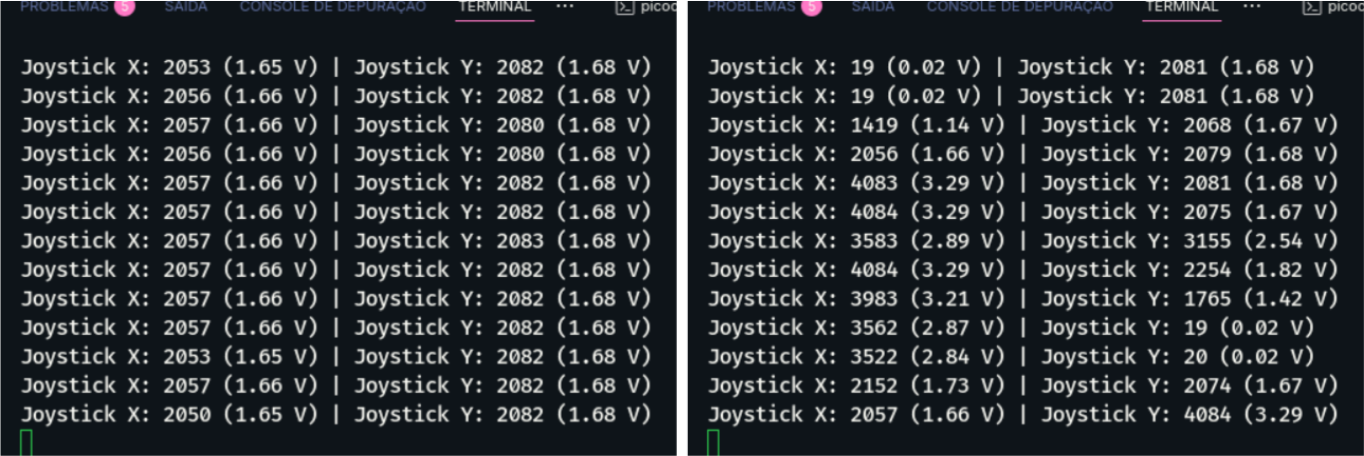
\includegraphics[width=0.8\textwidth]{fig/valores_loystick.png}
    \caption{Valores lidos do joystick exibidos no terminal.}
    \label{fig:valores_joystick}
\end{figure}

e quando o joystick está na "posição inicial" o valor observado para x e para y são 1.66V e 1.68V respectivamente.

Para conseguir ler o tempo todo usamos a seguinte lógica:


\begin{verbatim}
    while (true) {
       uint16_t x_analog = read_analog(JOYSTICK_X);
       uint16_t y_analog = read_analog(JOYSTICK_Y);


       float x_volts = (x_analog / 4095.0) * 3.3;
       float y_volts = (y_analog / 4095.0) * 3.3;


       printf("Joystick X: %u (%.2f V) | Joystick Y: %u (%.2f V)\n", x_analog, x_volts, y_analog, y_volts);
       sleep_ms(500);
   }
\end{verbatim}


\section{PWM controlado pelo Joystick }

Os valores de frequência e duty observados variaram conforme o ajuste do joystick, que controla o ciclo de trabalho do PWM gerado pelo Raspberry Pi Pico foram:

\begin{figure}[h]
    \centering
    \begin{subfigure}{0.8\textwidth}
        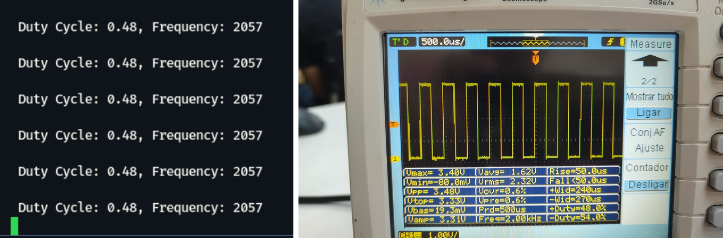
\includegraphics[width=\textwidth]{fig/osciloscopio_2k.png}
        \caption{Sinal PWM observado no osciloscópio com frequência de 2~kHz.}
        \label{fig:pwm_2k}
    \end{subfigure}
    \begin{subfigure}{0.8\textwidth}
        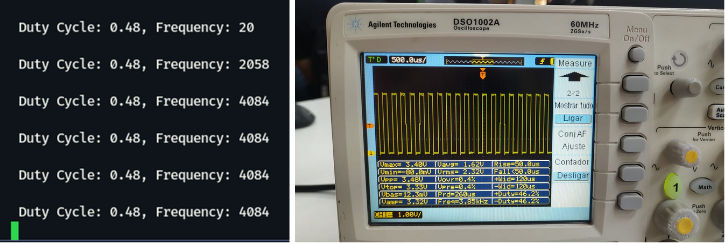
\includegraphics[width=\textwidth]{fig/osciloscopio_4k.png}
        \caption{Sinal PWM observado no osciloscópio com frequência de 4~kHz.}
        \label{fig:pwm_4k}
    \end{subfigure}
    \caption{Formas de onda PWM para diferentes posições do joystick.}
    \label{fig:pwm_osciloscopio}
\end{figure}


\section{Filtro RC e Conversão Digital–Analógica }
\subsection{Montagem}
Para a montagem do passa baixa, usamos um resistor de 9.9~k$\Omega$ e um capacitor de 101.5~$\mu$F

Logo, usando a formula do passa-baixa, temos que a frequência de corte é:

\[
    f_c = \frac{1}{2\pi R C} = \frac{1}{2 \pi \cdot 9.9 \cdot 10^3 \cdot 101.5 \cdot 10^{-9}} = 158 Hz
\]

Como o valor calculado é muito baixo, utilizamos um resistor de 1~k$\Omega$, onde obtemos uma frequância de corte nova no valor de ~1.6~k Hz, permitindo que a primeira harmônica não seja descartada pelo filtro, garantindo uma saída mais nítida.



Para o código, fizemos algumas pequenas modificações na \texttt{main}:

\begin{verbatim}
    
    while (true) {       
        duty += 0.1;
        if (duty > 1.09)
            duty = 0;
        
        configure_pwm(slice_num, channel, freq, duty);
        
        button_controller(GPIO_16, &status_button, &last_state, 1, 0);
        
        static absolute_time_t last_print_time = {0};
        if (absolute_time_diff_us(last_print_time, get_absolute_time()) >= 1000000) {
            printf("Duty Cycle: %.2f, Frequency: %d, GPIO Frequency: %d\n", duty, freq, status_button - counter);
            last_print_time = get_absolute_time();
            counter = status_button;
        }
        sleep_ms(3000);

    
        
    }
\end{verbatim}


Os valores medidos e esperados de tensão para cada duty se encontram na seguinte tabela, para 100uF, 1kOmega e 1000Khz.

\begin{table}[h!]
\centering
    \caption{Relação entre Duty Cycle, Tensões Medidas, Tensão Esperada e Erro}
    \begin{tabular}{|c|c|c|c|c|}
        \hline
        \textbf{Duty Cycle} & \textbf{Tensão de Entrada Osilocópio (V)} & \textbf{Vc Medido (V)} & \textbf{Tensão Esperada (V)} & \textbf{Erro (\%)} \\
        \hline
        0.1 & 0.280 & 0.290 & 0.33 & -14.29 \\
        0.2 & 0.610 & 0.630 & 0.66 & -4.92 \\
        0.3 & 0.945 & 0.970 & 0.99 & -2.11 \\
        0.4 & 1.27  & 1.30  & 1.32 & -1.57 \\
        0.5 & 1.6   & 1.64  & 1.65 & -0.63 \\
        0.6 & 1.93  & 1.97  & 1.98 & -0.52 \\
        0.7 & 2.26  & 2.30  & 2.31 & -0.44 \\
        0.8 & 2.59  & 2.63  & 2.64 & -0.39 \\
        0.9 & 2.92  & 2.97  & 2.97 & 0.00 \\
        1.0 & 3.25  & 3.31  & 3.30 & 0.31 \\
        \hline
    \end{tabular}
    \label{tab:duty_tensao}
\end{table}

\begin{figure}[H] 
    \centering
    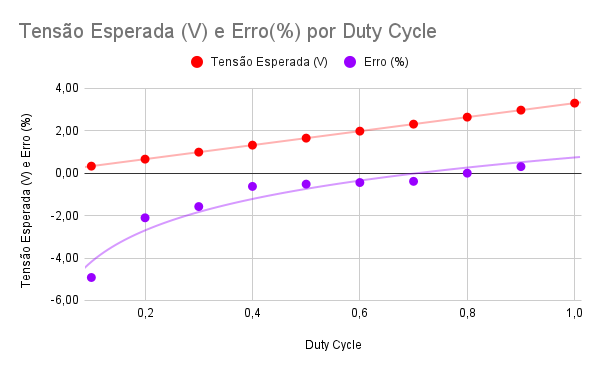
\includegraphics[width=14cm]{fig/grafico.png}
    \label{fig:grafico}
\end{figure}

O circuito usado para essas medições foi o que se encontra na Figura \ref{fig:circuito}.

\begin{figure}[H] 
    \centering
    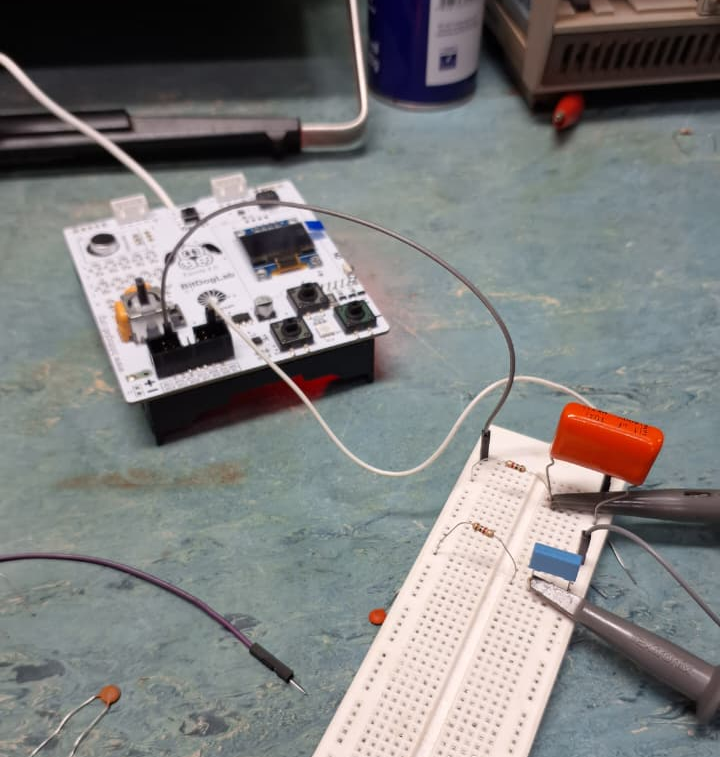
\includegraphics[width=0.3\textwidth]{fig/circuito.jpeg}
    \caption{Circuito utilizado para a conversão digital–analógica via filtro RC, composto por resistor de 1~k$\Omega$ e capacitor de 100~$\mu$F, conectado à saída PWM do Raspberry Pi Pico.}
    \label{fig:circuito}
\end{figure}


\section{Conclusão e Comentários}

Os resultados obtidos confirmam a relação teórica entre o ciclo de trabalho do sinal PWM e a tensão média medida após a filtragem pelo circuito RC. 
Observamos que, para baixos valores de duty cycle, o erro relativo foi mais significativo, chegando a cerca de --14\%, mas rapidamente se estabilizou com valores próximos a zero para duty cycles acima de 0.5. 
Isso se explica pela limitação prática do filtro RC, que apresenta uma resposta mais imprecisa em tensões muito baixas devido ao tempo de carga e descarga do capacitor.

Outro ponto relevante é que a frequência de corte calculada (1.6k~Hz) se mostrou adequada para suavizar o sinal PWM de 1k~Hz, aproximando-o de uma tensão contínua. Ainda assim, pequenas ondulações (ripple) podem ser observadas, especialmente em duty cycles intermediários, evidenciando que um filtro de ordem maior poderia reduzir ainda mais esse efeito.

Adicionalmente, verificamos que ao diminuir a capacitância do filtro RC, o ripple observado no sinal de saída tornou-se mais "íngreme" e visível no osciloscópio. Esse comportamento está de acordo com a teoria: quanto menor a capacitância, menor a constante de tempo $\tau = RC$, e portanto menor a capacidade do capacitor de armazenar carga entre os pulsos do PWM. Como consequência, o capacitor se carrega e descarrega mais rapidamente, resultando em uma variação de tensão mais acentuada entre os ciclos, o que aumenta o ripple. Esse efeito de carga e descarga pode ser observado na Figura \ref{fig:100nF_1uF}, onde mantivemos o mesmo circuito variando a capacitância de 100~nF (linha amarela) para 1~$\mu$F (linha verde), para isso mantivemos a menor frequência de corte entre as duas frequências de corte. Além disso, subimos a frequência para ser superior à frequência de corte do circuito com o capacitor de 1~$\mu$F e o resultado pode ser observado na Figura \ref{fig:1uF}, mantendo em ambas um resitor de 1K$\Omega$.



\begin{figure}[H]
    \centering
    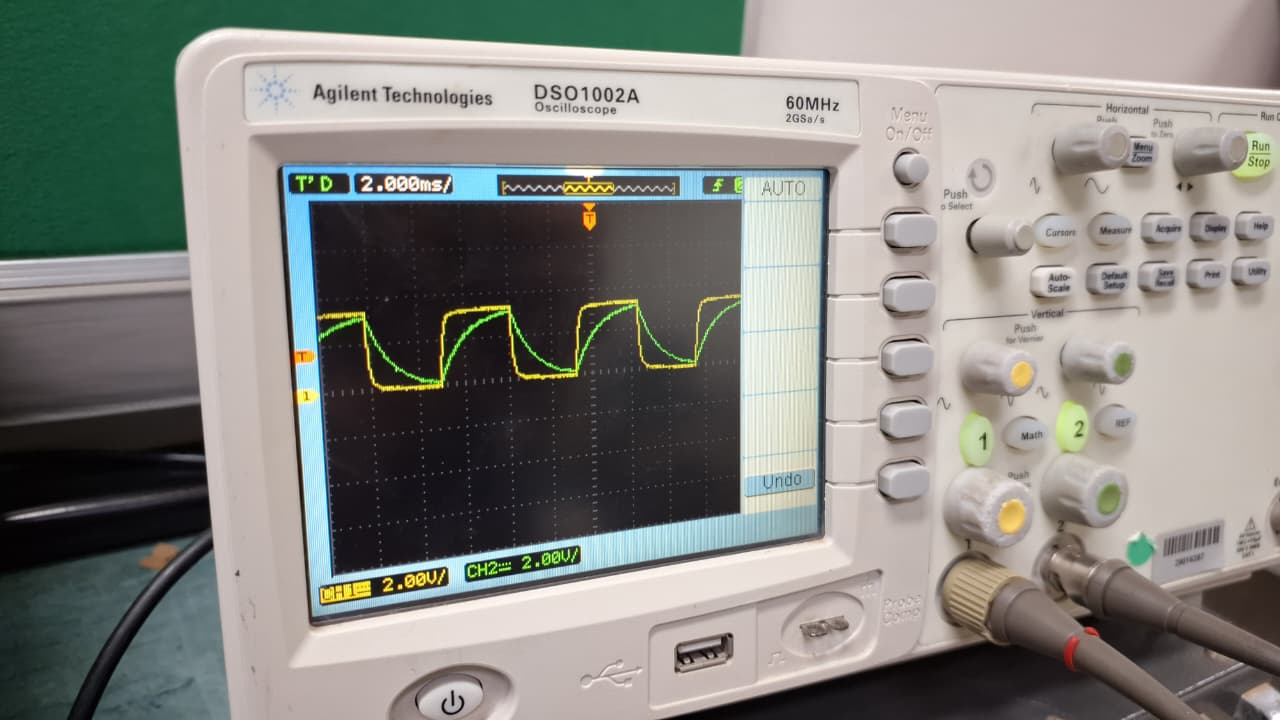
\includegraphics[width=0.6\textwidth]{fig/100nF_1uF.jpeg}
    \caption{Comparação do ripple na saída do filtro RC para capacitâncias de 100~nF (linha amarela) e 1~$\mu$F (linha verde), mantendo o mesmo circuito e frequência de corte. Observa-se que o ripple é mais acentuado para o capacitor de menor valor.}
    \label{fig:100nF_1uF} 
\end{figure}
 

\begin{figure}
    \centering
    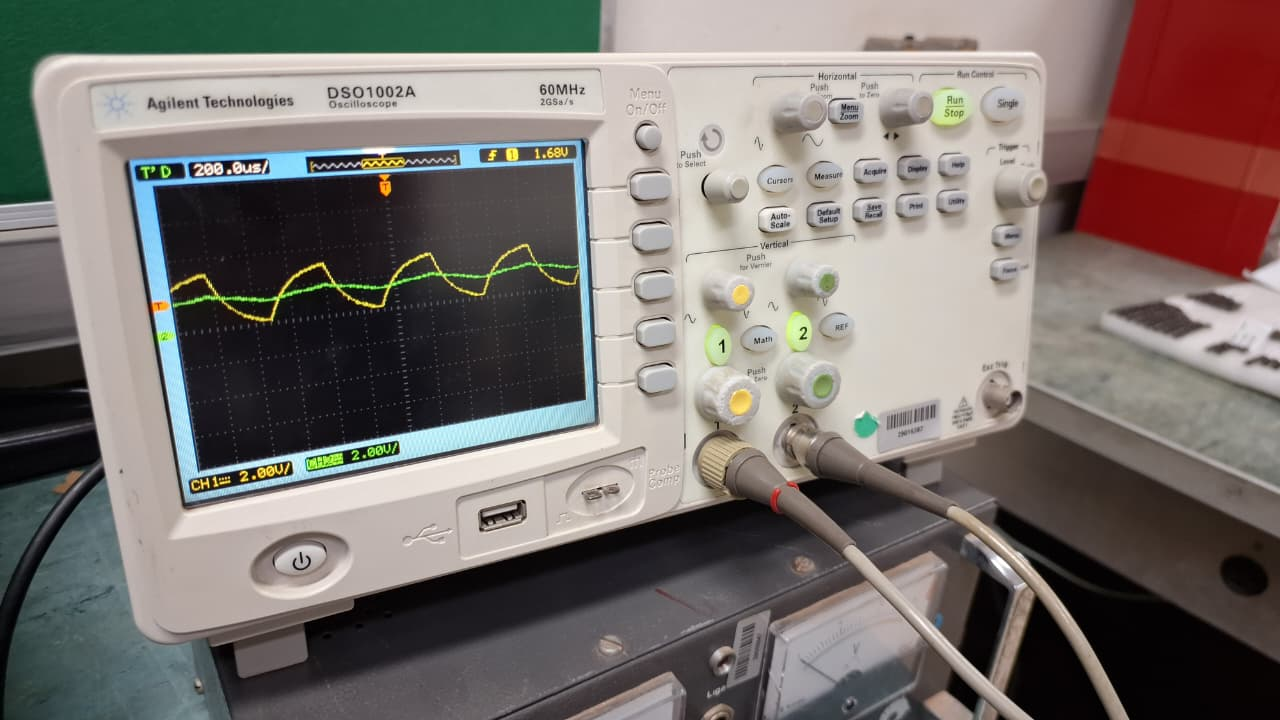
\includegraphics[width=0.6\textwidth]{fig/1uF.jpeg}
    \caption{Forma de onda observada na saída do filtro RC com capacitor de 1~$\mu$F, utilizando uma frequência de PWM acima da frequência de corte. O sinal apresenta menor ripple, aproximando-se de uma tensão contínua.}
    \label{fig:1uF}
\end{figure}


Além disso, o controle 1~via joystick se mostrou funcional, permitindo variar o duty cycle do PWM e observar diretamente o impacto no valor médio da tensão de saída. Esse tipo de implementação ilustra bem a transição entre o domínio digital e o analógico, destacando a importância dos conversores e filtros em sistemas embarcados.

\subsection*{Comentários finais}
\begin{itemize}
    \item O uso do BitDogLab simplificou a prototipagem, permitindo integrar rapidamente leitura analógica, geração de PWM e medição dos resultados.
    \item O osciloscópio foi essencial para validar o comportamento real do sinal, mostrando que, apesar da teoria prever valores ideais, fatores como a tolerância dos componentes e o ripple afetam os resultados.
    \item A análise do efeito da capacitância no filtro evidenciou a importância de escolher valores adequados para reduzir o ripple e aproximar o sinal do valor médio esperado.
    \item Como sugestão de melhoria, poderia ser testado um filtro ativo ou de segunda ordem, a fim de obter uma aproximação ainda mais fiel entre o valor esperado e o medido.
\end{itemize}

Em conclusão, o experimento demonstrou com clareza a conversão de sinais digitais em analógicos por meio de PWM e filtragem RC, reforçando conceitos fundamentais de eletrônica e sistemas embarcados.



\end{document}